\section{Differentiating inverse functions}

\begin{definition}
If a function $f$ is one-to-one, we can find its \textbf{inverse}, $f^{-1}$. The inverse satisfies $$f^{-1}(f(x))=x$$ for all values of $x$ in the domain of $f$.
\end{definition}

This notation is most commonly used for trigonometric functions ($\sin^{-1}$, $\cos^{-1}$ and $\tan^{-1}$.).

\note{$\tan^{-1}x$ is used for the inverse of $\tan$ and NOT $\frac{1}{\tan x}$.}

\note{Sometimes, $\arcsin$, $\arccos$ and $\arctan$ are used to represent $\sin^{-1}$, $\cos^{-1}$ and $\tan^{-1}$.}

\begin{thing}{Finding the derivative of an inverse}
Let $f$ be a function. The derivative of $f^{-1}$ is:
$$\frac{d}{dx}\left(f^{-1}(x)\right)=\frac{1}{f'(f^{-1}(x))}$$
\begin{proof}
Let $f$ be a function and let $g=f^{-1}$. By the chain rule,
$$\frac{d}{dx} f(g(x)) = f'(g(x))g'(x).$$
$g$ is $f^{-1}$, so $f(g(x))=x$ and $$\frac{d}{dx} f(g(x)) = 1.$$
Therefore, $$1 = f'(g(x))g'(x).$$ Rearranging gives $$g'(x)=\frac{1}{f'(g(x))}.$$
\end{proof}
\end{thing}

The method in the proof can be used to differentiate inverse functions:

\begin{example}
To find 
$$\frac{d}{dx}\left(\sin^{-1}x\right),$$
we first look at
\begin{align*}
\frac{d}{dx}\left(\sin\left(\sin^{-1}x\right)\right)&=\frac{d}{dx}\left(x\right)\\
&=1.
\end{align*}
Using the chain rule,
$$\frac{d}{dx}\left(\sin\left(\sin^{-1}x\right)\right)=\cos\left(\sin^{-1}x\right)\cdot\frac{d}{dx}\left(\sin^{-1}x\right).$$
Therefore:
$$\cos\left(\sin^{-1}x\right)\cdot\frac{d}{dx}\left(\sin^{-1}x\right)=1$$
$$\frac{d}{dx}\left(\sin^{-1}x\right)=\frac{1}{\cos\left(\sin^{-1}x\right)}$$

We can simplify this, by letting $\theta=\sin^{-1}x$, then looking at the following triangle:
\begin{figure}[H]
\centering
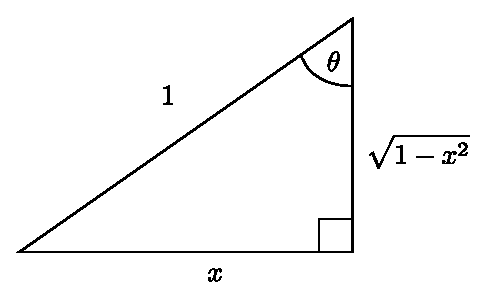
\includegraphics[scale=0.8]{img/right-angle-tri-arcsin}
\captionstyle{\centering\it}
\caption{$\sin(\theta)=x$}
\label{fig:right-angle-tri-arcsin}
\end{figure}

This tells us that $\cos\theta = \sqrt{1-x^2}$. Therefore
$$\frac{d}{dx}\left(\sin^{-1}x\right)=\frac{1}{\sqrt{x^2-1}}.$$

\end{example}

We can also find the derivatives of inverses by using:
\begin{in_a_box}
$$\frac{dy}{dx}=\frac{1}{\frac{dx}{dy}}$$
\end{in_a_box}

\begin{example}
To find 
$$\frac{d}{dx}\left(\sin^{-1}x\right),$$
let $y=\sin^{-1}x$. This means that $x=\sin y$ and so:
$$\frac{dx}{dy}=\cos y$$
\begin{align*}
\frac{dy}{dx}&=\frac{1}{\frac{dx}{dy}}\\
&=\frac{1}{\cos y}\\
&=\frac{1}{\cos\left(\sin^{-1}x\right)}
\end{align*}

Simplifying as before gives
$$\frac{d}{dx}\left(\sin^{-1}x\right)=\frac{1}{\sqrt{x^2-1}}.$$

\end{example}


\begin{example}
\begin{align*}
\frac{d}{dx}\left(\cos^{-1}x\right)&=-\frac{1}{\sin(\cos^{-1}x)}\\
&=-\frac{1}{\sqrt{1-x^2}}
\end{align*}
\end{example}
\begin{example}
\begin{align*}
\frac{d}{dx}\left(\tan^{-1}x\right)&=\frac{1}{1+\tan^2(\tan^{-1}x)}\\
&=\frac{1}{1+x^2}
\end{align*}
\end{example}
